\newpage
\section{Leitner's Box GUI}
\genHeader

We would like to now provide you with a simple GUI with which you can take your model for a spin and see it in action.

\begin{itemize}

\item[$\blacktriangleright$] Navigate to the top left of your toolbar and start the ``New'' wizard.

\item[$\blacktriangleright$] Load ``Examples/eMoflon Handbook Examples/Part II GUI Download'' (Fig.~\ref{eclipse:GUI_load}). This will load the new project
into your workspace.\footnote{If nothing appears, go to the small arrow to the right of the window, and select ``Configure Working Sets\ldots'' Make sure
\texttt{Other Projects} is selected, and press \texttt{Ok}.} Right click \texttt{LeitnersBox} to invoke the context menu and select ``Run as/Java application.''

\begin{figure}[htbp]
    \centering
    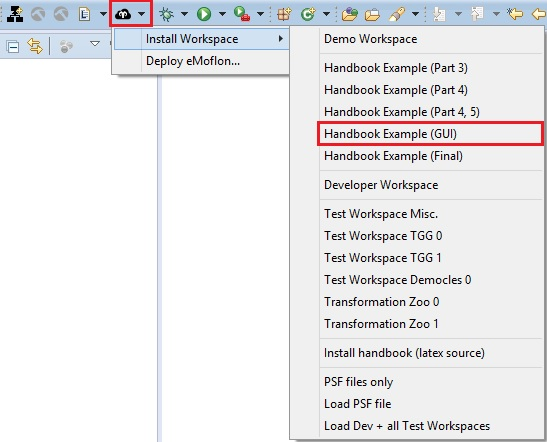
\includegraphics[width=0.7\textwidth]{eclipse_loadGUI}
    \caption{Load Leitner's Box GUI}
    \label{eclipse:GUI_load}
\end{figure}

\clearpage

\item[$\blacktriangleright$] The GUI will automatically navigate to the instances folder where you've stored your instance model, then load your partitions and
cards into the visualized box. Please note that this will only work if you named your dynamic instance \texttt{Box.xmi} and placed it in the \texttt{instances}
folder as suggested.

\vspace{0.5cm}

\item[$\blacktriangleright$] Navigate to any card, and you'll be able to see two options, ``Remove Card'' and ``Check Card''
(Fig~\ref{eclipse:GUI_cardOptions}). While we'll implement ``Check Card" in Part III, ``Remove Card'' is currently active, implemented by the injection you
just created.

\vspace{1cm}

\begin{figure}[htbp]
    \centering
    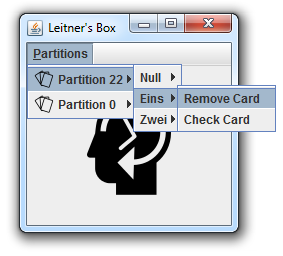
\includegraphics[width=0.5\textwidth]{eclipse_GUICardOptions}
    \caption{Using the GUI with your instance}
    \label{eclipse:GUI_cardOptions}
\end{figure}

\vspace{1cm}

\item[$\blacktriangleright$] Experiment with your instance model and confirm your injection works by removing some items from the GUI.  You'll notice the change
immediately in the \texttt{Box.xmi} file. You can also close the GUI and add, remove, or rename more elements in the model, then observe how the changes are
reflected in the GUI.

\vspace{0.5cm}

\item[$\blacktriangleright$] Expand the ``Other Projects" node and explore \texttt{LeitnersBoxController} and \texttt{LeitnersBoxView} files to get an
understanding of the GUI. Can you find where the controller loads and connects to the model?

\end{itemize}
